\chapter{他のブロックを作る}
\section{LBlockクラス}
今までのTブロックを元に、Lブロックを作ります。
\begin{figure}[h]
  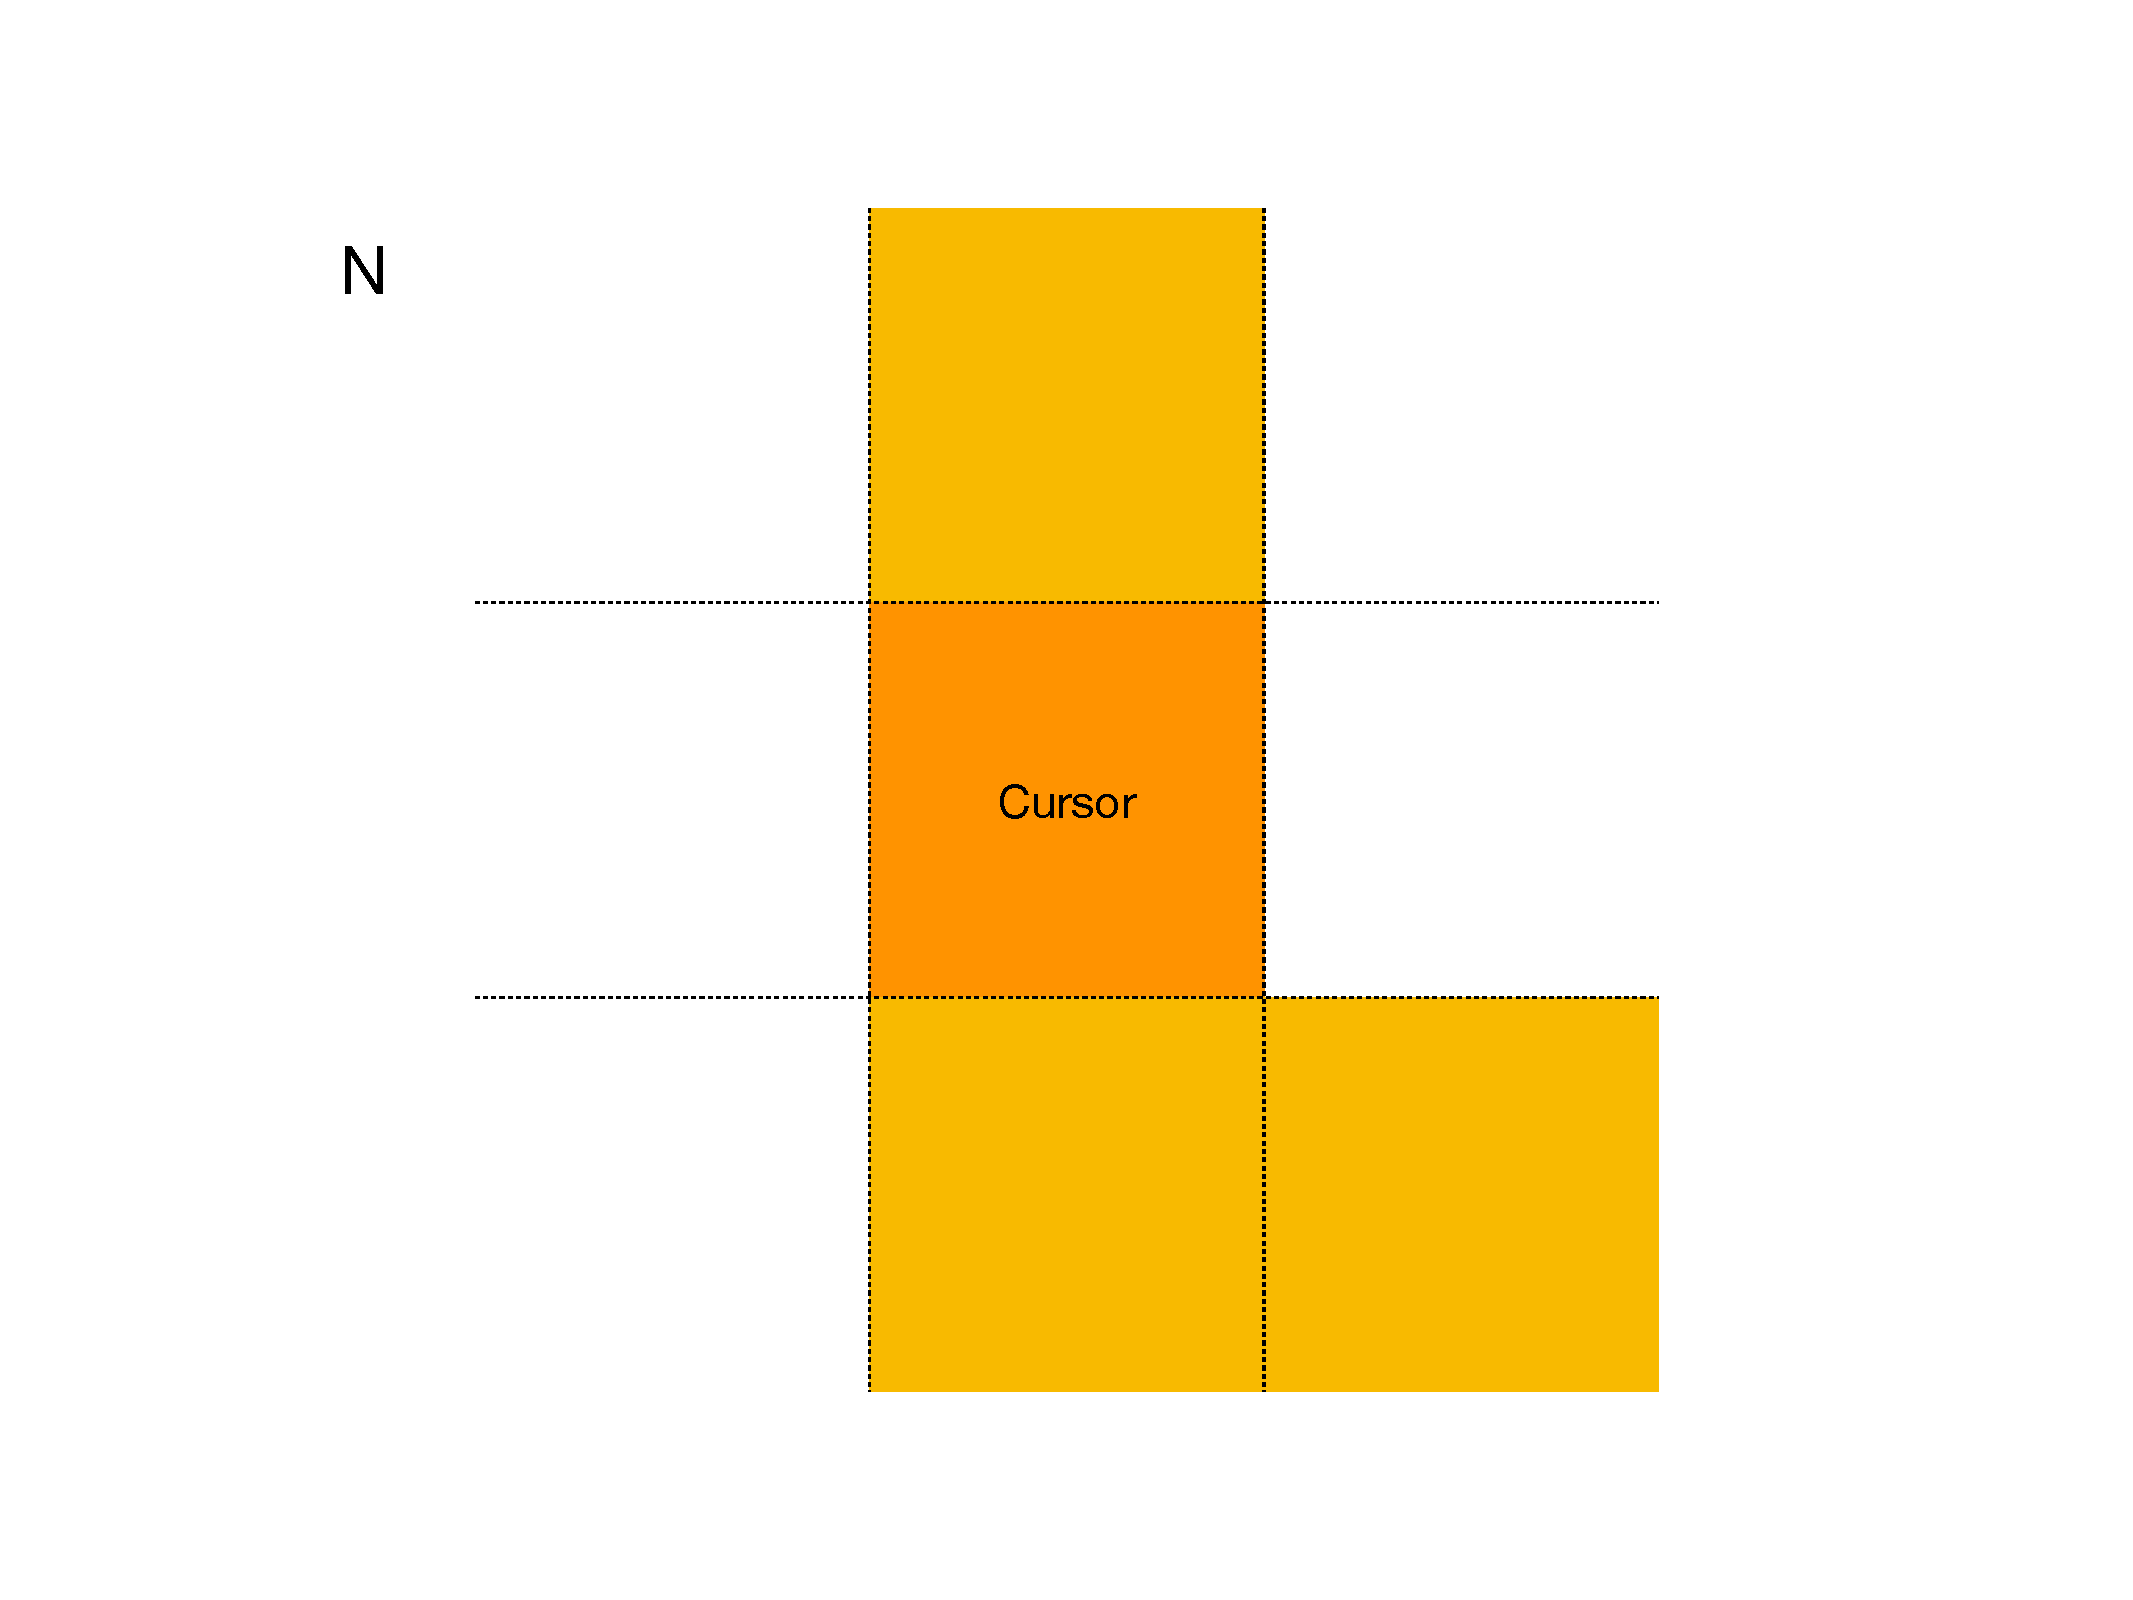
\includegraphics[width=60mm, page=1]{images/LBlock.pdf}
  \includegraphics[width=60mm, page=2]{images/LBlock.pdf}
  \includegraphics[width=60mm, page=3]{images/LBlock.pdf}
  \includegraphics[width=60mm, page=4]{images/LBlock.pdf}
  \caption{Lブロック}
\end{figure}
クラス名はLBlockとしましょう。色はオレンジが多いようです。
以下の関数を作るのを忘れないでください。
\begin{itemize}
  \item block\_info関数 ... カーソルの位置から自分のブロックの様子を座標のリストで返します。
  \item rotate関数 ... 回転します。回転できるかは気にせず、とりあえずselfに入っているrotationという変数を変えるだけにします。
  \item can\_rotate関数 ... 実際に回転したときにはみ出さないか、他のブロックとぶつからないか判定します。引数cursorで現在の位置を、引数board\_infoで盤面の情報を取得します。
  \item can\_go\_up関数 ... 上に移動できるか判定します。引数cursorで現在の位置を、引数board\_infoで盤面の情報を取得します。
  \item can\_go\_down関数 ... 下に移動できるか判定します。引数cursorで現在の位置を、引数board\_infoで盤面の情報を取得します。
  \item can\_go\_right関数 ... 右に移動できるか判定します。引数cursorで現在の位置を、引数board\_infoで盤面の情報を取得します。
  \item can\_go\_left関数 ... 左に移動できるか判定します。引数cursorで現在の位置を、引数board\_infoで盤面の情報を取得します。
\end{itemize}
出来上がったら、main関数で表示してみましょう。
main.pyのmoving\_block = の部分を変更したらできるはずです。

\section{JBlockクラス}
次にJブロックを作ります。
\begin{figure}[h]
  \includegraphics[width=60mm, page=9]{images/Blocks.pdf}
  \includegraphics[width=60mm, page=10]{images/Blocks.pdf}
  \includegraphics[width=60mm, page=11]{images/Blocks.pdf}
  \includegraphics[width=60mm, page=12]{images/Blocks.pdf}
  \caption{Jブロック}
\end{figure}
関数も同じものを作ります。
自分を信じすぎず、一つブロックを作ったらきちんと表示、回転、移動ができるか確認しましょう。

\newpage
\section{SBlockクラス}
次にSブロックを作ります。
\begin{figure}[h]
  \includegraphics[width=60mm, page=13]{images/Blocks.pdf}
  \includegraphics[width=60mm, page=14]{images/Blocks.pdf}
  \includegraphics[width=60mm, page=15]{images/Blocks.pdf}
  \includegraphics[width=60mm, page=16]{images/Blocks.pdf}
  \caption{Sブロック}

\end{figure}
関数も同じものを作ります。

\newpage
\section{ZBlockクラス}
次にZブロックを作ります。
\begin{figure}[h]
  \includegraphics[width=60mm, page=17]{images/Blocks.pdf}
  \includegraphics[width=60mm, page=18]{images/Blocks.pdf}
  \includegraphics[width=60mm, page=19]{images/Blocks.pdf}
  \includegraphics[width=60mm, page=20]{images/Blocks.pdf}
  \caption{Zブロック}
\end{figure}

\newpage
\section{IBlockクラス}
最後にIブロックを作ります。
\begin{figure}[h]
  \includegraphics[width=60mm, page=21]{images/Blocks.pdf}
  \includegraphics[width=60mm, page=22]{images/Blocks.pdf}
  \includegraphics[width=60mm, page=23]{images/Blocks.pdf}
  \includegraphics[width=60mm, page=24]{images/Blocks.pdf}
  \caption{Iブロック}
\end{figure}
うまく動いていることが確認できたでしょうか。
ブロックはこれで全てです。お疲れ様でした。
